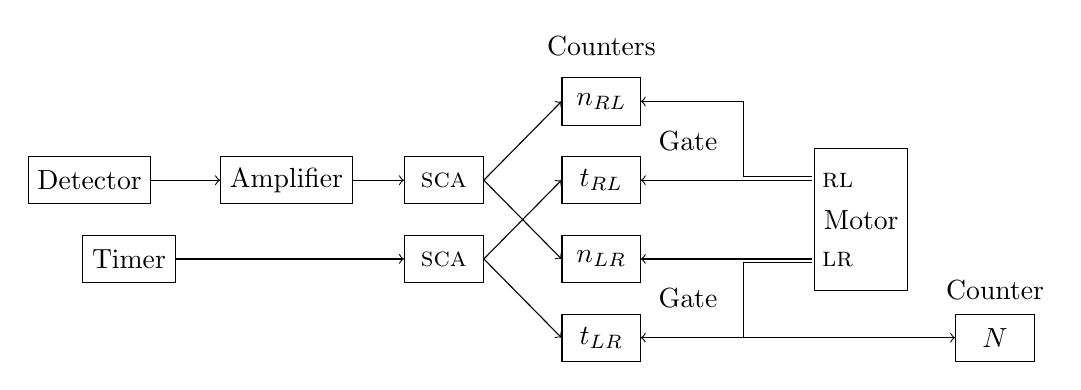
\begin{tikzpicture}[
rect/.style={
draw,
minimum height=.6cm,
minimum width=1.cm,
},
]
    \node (det) at (-0.5,.5) [rect] {Detector};
    \node (amp) at (2,.5) [rect] {Amplifier};
    \node (sca_det) at (4,.5) [rect] {\textsc{sca}};
    \node (timer) at (0,-.5) [rect] {Timer};
    \node (sca_timer) at (4,-.5) [rect] {\textsc{sca}};

    \draw[->] (det) to (amp);
    \draw[->] (amp) to (sca_det);
    \draw[->] (timer) to (sca_timer);

    \node  at (6,2.2)  {Counters};
    \node (NRL) at (6,1.5) [rect] {$n_\text{RL}$};
    \node (TRL) at (6,0.5) [rect] {$t_\text{RL}$};
    \node (NLR) at (6,-.5) [rect] {$n_\text{LR}$};
    \node (TLR) at (6,-1.5) [rect] {$t_\text{LR}$};

    \draw[->] (sca_det.east) to (NRL.west);
    \draw[->] (sca_det.east) to (NLR.west);
    \draw[->] (sca_timer.east) to (TRL.west);
    \draw[->] (sca_timer.east) to (TLR.west);

    \node (RL) at (9.,.5) [] {\textsc{rl}};
    \node (motor) at (9.3,0) [draw, minimum height=1.8cm] {Motor};
    \node (LR) at (9.,-.5) [] {\textsc{lr}};

    \node at (11.,-.9) {Counter};
    \node (counter) at (11.,-1.5) [rect] {$N$};

    \node at (7.1,1) {Gate};
    \node at (7.1,-1) {Gate};

    \draw[->] (8.68,.55) -- (7.8,.55) -- (7.8,1.5) to (6.5,1.5);
    \draw[->] (8.68,.5) to (6.5,.5);

    \draw[->] (8.68,-.55) -- (7.8,-.55) -- (7.8,-1.5) to (6.5,-1.5);
    \draw[->] (7.8,-1.5) to (counter);
    \draw[->] (8.68,-.5) to (6.5,-.5);
\end{tikzpicture}
